\chapter{Exercise 07}
\extitle{Practicing Ridge Regression}
%%******************************************************************************%
%                                                                              %
%                                 Interlude                                    %
%                         for Machine Learning module                          %
%                                                                              %
%******************************************************************************%

% =============================================== %
\section*{Interlude - Introducing Polynomial Models}
% ----------------------------------------------- %

You probably noticed that the method we use is called \textit{linear regression} for a reason:
the model generates all of its predictions on a straight line.
However, we often encounter features that do not have a linear relationship with the predicted variable,
like in the figure below:

\begin{figure}[!h]
    \centering
    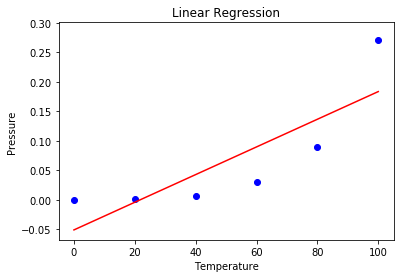
\includegraphics[scale=0.6]{assets/polynomial_straight_line.png}
    \caption{Non-linear relationship}
\end{figure}

In that case, we are stuck with a straight line that cannot fit the data points properly.
In this example, what if we could express $y$ not as a function of $x$, but also of $x^2$, and maybe even $x^3$ and $x^4$?
We could make a hypothesis that draws a nice \textbf{curve} that would better fit the data.
That's where polynomial features can help!

% =============================================== %
\section*{Interlude - Polynomial features}
% ----------------------------------------------- %
First we get to do some \textit{feature engineering}.
We create new features by raising our initial $x$ feature to the power of 2, and then 3, 4... as far as we want to go.
For each new feature we need to create a new column in the dataset.

% =============================================== %
\section*{Interlude - Polynomial Hypothesis}
% ----------------------------------------------- %
Now that we created our new features, we can combine them in a linear hypothesis that looks just the same as what we're used to:

$$
\hat{y} = \theta_0 + \theta_1 x  +\theta_2 x^{2} + \dots + \theta_n x^{n}
$$  

It's a little strange because we are building a linear combination, not with different features but with different powers of the same feature.
This is a first way of introducing non-linearity in a regression model!
%\newpage
\turnindir{ex07}
\exnumber{07}
\exfiles{space\_avocado.py, benchmark\_train.py,  models.[csv/yml/pickle]}
\exforbidden{sklearn}
\makeheaderfilesforbidden


% ================================= %
\section*{Objective}
% --------------------------------- %
It's training time!  
Let's practice our brand new Ridge Regression with a polynomial model.

% ================================= %
\section*{Introduction}
% --------------------------------- %
You have already used the dataset \texttt{space\_avocado.csv}.
The dataset is constituted of 5 columns:
\begin{itemize}
  \item \textbf{index}: not relevant,
  \item \textbf{weight}: the avocado weight order (in ton),
  \item \textbf{prod\_distance}: distance from where the avocado ordered is produced (in Mkm),
  \item \textbf{time\_delivery}: time between the order and the receipt (in days),
  \item \textbf{target}: price of the order (in trantorian unit).
\end{itemize}
It contains the data of all the avocado purchase made by Trantor administration (guacamole is a serious business there).

% ================================= %
\section*{Instructions}
% --------------------------------- %
You have to explore different models and select the best you find.
To do this:
\begin{itemize}
  \item Split your \texttt{space\_avocado.csv} dataset into a training, a cross-validation and a test sets.
  \item Use your \texttt{polynomial\_features} method on your training set.
  \item Consider several Linear Regression models with polynomial hypotheses with a maximum degree of $4$.
  \item For each hypothesis consider a regularized factor ranging from $0$ to $1$ with a step of $0.2$.
  \item Evaluate your models on the cross-validation set.
  \item Evaluate the best model on the test set.
\end{itemize}

According to your model evaluations, what is the best hypothesis you can get?
\begin{itemize}
  \item Plot the evaluation curve which help you to select the best model (evaluation metrics vs models + $\lambda$ factor).
  \item Plot the true price and the predicted price obtain via your best model with the different $\lambda$ values (meaning the dataset + the 5 predicted curves).
\end{itemize}


The training of all your models can take a long time.
Thus you need to train only the best one during the correction.
But, you should return in \texttt{benchmark\_train.py} the program which perform the training of all the models and save the parameters of the different models into a file.
In \texttt{models.[csv/yml/pickle]} one must find the parameters of all the models you have explored and trained.
In \texttt{space\_avocado.py} train the model based on the best hypothesis you find and load the other models from \texttt{models.[csv/yml/pickle]}.
Then evaluate the best model on the right set and plot the different graphics as asked before.
